%%%%%%%%%%%%%%%%%%%%%%%%%%%%%%%%%%%%%%%%%%%%%%%%%%%%%%%%%%%%%%%%%%%
%
% This is a general template file for the LaTeX package SVJour3
% for Springer journals.          Springer Heidelberg 2010/09/16
%
% Copy it to a new file with a new name and use it as the basis
% for your article. Delete % signs as needed.
%
% This template includes a few options for different layouts and
% content for various journals. Please consult a previous issue of
% your journal as needed.
%
%%%%%%%%%%%%%%%%%%%%%%%%%%%%%%%%%%%%%%%%%%%%%%%%%%%%%%%%%%%%%%%%%%%
%
\RequirePackage{fix-cm}
%
\documentclass[twocolumn]{svjour3}
%
\smartqed
%
\usepackage{graphicx}
\usepackage[T1]{fontenc}
\usepackage{hyperref}
\usepackage[round, sort&compress, numbers]{natbib}
\usepackage{multirow}
\usepackage{graphicx}
\usepackage{units}
\usepackage{color}
\usepackage{colortbl}
\usepackage{xspace}
%
\DeclareRobustCommand\IPCClongname{}
\setcounter{secnumdepth}{5}
%
% please place your own definitions here and don't use \def but \newcommand{}{}
\newcommand{\pmlib}{\texttt{pmlib}\xspace}
%
% Insert the name of "your journal" with
% \journalname{myjournal}
%
\begin{document}

\title{Evaluating the Performance and Energy Efficiency of the
  COSMO-ART model system}
%\thanks{}
%\subtitle{}

%\titlerunning{Short form of title} % if too long for running head

\author{Joseph~Charles \and William~Sawyer \and Manuel~F.~Dolz \and
  Sandra~Catal\'an}

%\authorrunning{Short form of author list} % if too long for running
%head

\institute{J.~Charles, W.~Sawyer
	\at Swiss National Supercomputing Centre (CSCS)
	\\ CH-6900 Lugano, Switzerland
 	\\ E-mails:~{\{joseph.charles,william.sawyer\}@cscs.ch}
        \and M.~F.~Dolz
        \at Dept. of Informatics, University of Hamburg (UHAM)
	\\ DE-22527 Hamburg, Germany
        \\ \email{manuel.dolz@informatik.uni-hamburg.de}
        \and S.~Catal\'an
        \at Jaume I University of Castell\'on (UJI)
	\\ ES-12071 Castell\'on, Spain
        \\ \email{catalans@icc.uji.es}
}

\date{Received: date / Accepted: date} % The correct dates will be
                                       % entered by the editor

\maketitle

\begin{abstract}
  In this  paper we investigate  the energy footprint  and performance
  profiling of COSMO-ART  on various HPC platforms.  This  model is an
  extension of  the operational weather  forecast model of  the German
  weather  service   (DWD),  developed  for  the   evaluation  of  the
  interactions of reactive gases  and aerosol particles with the state
  of atmosphere at the  regional scale.  Different measurement devices
  and energy-aware techniques are  described to evaluate both time and
  energy  to  solution  of  the  considered application  and  to  gain
  detailed  insights  into power  and  performance requirements.   Our
  motivation  is to  improve  corresponding code  sections to  sustain
  performance  while minimising energy-to-solution.   This preliminary
  work  sets the  basis for  subsequent studies  to  tackle challenges
  related  to  energy  efficient  high performance  computing  in  the
  framework of the Exa2Green project (\url{http://exa2green.eu/}).

\keywords{High performance computing  \and Energy-aware computing \and
  Green computing  \and Numerical weather  prediction \and Atmospheric
  chemistry  \and  Aerosols  modelling  \and  Profiling  methods  \and
  Benchmark    analysis   \and    COSMO-ART    coupled   model    \and
  Time-to-solution \and Energy-to-solution \and Xeon processor}
% \PACS{PACS code1 \and PACS code2 \and more}
% \subclass{MSC code1 \and MSC code2 \and more}
\end{abstract}

\section{Introduction}
\label{intro}
While anthropogenic greenhouse gas emissions are driving unprecedented
major  climate  changes  since   the  mid-20$^{th}$  Century,  one  factor
overwhelmingly  affects  the  uncertainty  in  determining  human-induced
radiative  forcing:  the  effects   of  aerosols  in  the  atmosphere.
Although they  are not considered  heat-trapping greenhouse  gases and
have  shorter  atmospheric lifetimes,  aerosols  significantly modify  the
global   radiation   budget   \citep{IPCC-2013}.   Enhanced   aerosols
concentrations impact the climate  system by scattering and absorption
of solar radiation, thereby exerting a direct radiative forcing; or by
modifying cloud  properties,  cloud  fraction and  surface
albedo,  causing  a  negative  indirect  radiative  forcing.   Despite
considerable  progress in  global aerosol  modelling \citep{Mann-2013}
and  measurement-based  assessments,  large  uncertainties  remain  in
current  estimates  of  aerosol radiative  forcing  \citep{Myhre-2013,
IPCC-2013,  Lee-2013,   Randles-2013,  Rosenfeld-2013,  Sherwood-2013,
Stier-2013}.

Hence to  improve our understanding of  aerosol-cloud interactions and
reduce  these  uncertainties,  the  research  community  is  making  a
concerted international  effort to represent  the underlying physical,
chemical  and aerosol dynamical  processes through  numerical chemical
transport  models (CTMs)  such  as ART  (Aerosols  and Reactive  Trace
gases),   developed   at  the   Karlsruhe   Institute  of   Technology
(KIT)  \citep{Vogel-2009,  Bangert-2011,  Knote-2013}.  This  regional
scale modelling system is coupled  with the operational  weather forecast
model  \textsc{Cosmo}  \citep{Baldauf-2011},  jointly developed and used by  a
consortium of European weather centers, as well as utilised in a climate version
by the wider research community.

The extended  atmospheric model \textsc{Cosmo-art}  is com\-put\-ationally
much  more  demanding than  \textsc{Cosmo}  since  a  large number  of
additional  tracers and  processes have  to be  considered.   Thus the
model  is currently  severely limited  in terms  of applicability  and
expensive in terms of energy consumption.  Although \textsc{Cosmo} has
recently been ported to GPUs \citep{Gysi-2014, Lapillonne-2014} within
the framework of the  High Performance and High Productivity Computing
(HP2C) Initiative  \citep{HP2C} to optimise it  for computational and
energy efficiency,  significant investments in ART  are still required
to take it  to a similar level.  The  efficiency of \textsc{Cosmo-art}
is being  addressed in the  EU Exa2Green project  \citep{EXA2GREEN} to
deliver a  prototype code, which  provides an energy efficiency  of at
least five times the  baseline value.  Such an implementation would
allow  the  community  to  investigate critical  questions  at  higher
resolution  and   over  longer  periods,   at  reduced  cost   to  the
environment.

This  work is  organized as  follows: in  Sec.~\ref{sec:1} we  give an
overview  of  related  work,   then  in  Sec.~\ref{sec:2}  we  briefly
introduce \textsc{Cosmo-art}  and specify its  technical setup related
to  the investigated  performance and  energy evaluation  methods.  In
Sec.~\ref{sec:3}   we  describe   HPC  platforms,   power  measurement
equipments   and  software  environment   employed  to   conduct  this
benchmarking study.  Sec.~\ref{sec:4}  presents performance and energy
requirements  of the  baseline on  these architectures  and highlights
areas where improvements will be necessary for the subsequent baseline
refactoring.   Finally,  we  conclude in Sec.~\ref{concl} with some 
implications for the Exa2Green project and give an outlook for future
research.


\section{Related work \emph{(to be completed)}}
\label{sec:1}
While the  TOP500 list was  introduced over 20  years ago to  rank the
performance of HPC systems worldwide, it is quite recently that energy
efficiency  become  a  critical  constraint  in the  way  to  exascale
computing.   Since 2007,  the Green500  power  measurement methodology
encourages the design,  procurement and management of energy-efficient
infrastructures   to  contain   performance  in   an   affordable  and
competitive  power envelope.   However, the  state-of-the-art research
assessing performance  and energy efficiency of  applications is still
scarce.

\emph{Padoin et al.}   \cite{Padoin-2013} investigate performance and
power  consumption  of  an  agroforestry  application  and  show  that
changing workload  can drastically improve energy efficiency  of CPU +
GPU heterogeneous architectures.

\emph{Ou  Pang et  al.}   \cite{Ou-2012} compare  ARM  and Intel  x86
workstations  clusters  and   conclude  that  ARM-based  clusters  are
advantageous  with   lightweight  applications  in   terms  of  energy
efficiency.

\emph{G\"oddeke et al.}  \cite{Goddeke-2013} evaluate weak and strong
scalability of PDE solvers on a cluster of 96 ARM dual-core processors
and demonstrate  that the ARM-based  cluster can be more  efficient in
terms of energy-to-solution compared to x86-based cluster.

\emph{Wittmann  et  al.}   \cite{Wittmann-2013}  perform  a  thorough
analysis of  a lattice-Boltzmann method based CFD  simulation on Intel
Sandy   Bridge  processors   and  show   extrapolated  results   on  a
petascale-class machine.

% \emph{Cumming  et  al.}  \cite{Cumming-2014}  present  a simple  and
% practical  methodology  looking at  energy  minimization  that can  be
% applied to various applications.


\section{The COSMO-ART model system}
\label{sec:2}
\subsection{Model Description}
\label{subsec:1.1}

The model  system \cosmoart described  in \cite{Vogel-2009},
is  a  regional to  continental  scale  model  coupled online  to  the
\textsc{Cosmo}   numerical  weather   prediction  and   climate  model
\cite{Baldauf-2011}.   It   incorporates  sophisticated  modules  for
gaseous  chemistry   and  aerosol  dynamics  and   allows  the  online
calculation of  reactive trace  substances and their  interaction with
the  atmosphere.    Detailed  model   description  can  be   found  in
\cite{Bangert-2012, Knote-2011, Knote-2013}.

\subsection{Model Setup}
\label{subsec:1.2}

Establishing effective energy performance benchmarking of a code under
intense development  such as \cosmoart is  a challenging task
because of  the absolute necessity  that results must  be reproducible
within  an  expected  variance  for  the  duration  of  the  Exa2Green
pro\-je\-ct.  To   define  a  baseline,   it  was  necessary  to   find  a
run-configuration  capable  of   being  recreated  in  all  subsequent
versions.  Here  we give a brief  overview of the model  setup for our
performance and energy efficiency evaluation.

Three-dimensional simulations are performed over large parts of Europe
and the Mediterranean~Sea for April 13$^{th}$ 2010, near the equinox, in order to approximately
have a half  day  of  sun  exposure and  therefore  ensure  a typical
activation of the chemistry cycle.  The calculation domain corresponds
to the CORDEX-EU-44 domain and is covered by a grid of $222\times 216$
points with  a horizontal resolution of  $0.22\,^{\circ}$, i.e., 50~km
in  both directions  and 40~vertical  layers.  These  24-hour forecast
simulations  are not  preceded  by  a spin-up  phase  to build up  the
simulated gaseous and  aerosol concentrations.  This condition means 
that the model initialization needs a period of adjustment to reach its equilibrium  state and minimize  the effect of
initial conditions for gases and aerosols on the model predictions.

The meteorological initial and boundary conditions are obtained by the
the ECMWF  global spectral model IFS  with an update  frequency of 3h.
Boundary data  for gas-phase species are taken  from IFS-MOZART output
at  6h temporal resolution.   The model  setup incorporates  34~2D and
45~3D  fields to  be written  out  every hour  and is  devoid of  data
assimilation methods.

The considered  \cosmoart model  system is configured  with a
semi-Lagrangian    horizontal   advection    sche\-me    with   tricubic
interpolation  and selective filling  diffusion option  in combination
with   the   dynamical    core   using   Runge-Kutta   time   stepping
\cite{COSMO-PartI-2011}.    It  also   makes  use   of   the  Kinetic
PreProcessor solver (KPP) for  the solution of atmospheric chemistry
ordinary  differential equations \cite{Damian-2002}.   Concerning the
modelling  of  wet  deposition  in  aerosols, the  baseline  has  only
indirect  cloud feedbacks  but  does not  include in-cloud  scavenging
(rainout) and below-cloud  scavenging (washout) yet.  Amongst physical
parameterizations,   precipitation  formation   is   performed  by   a
two-moment cloud microphysics.


\section{Power-performance measurement framework}
\label{sec:3}
In this section,  we present three different frameworks  deployed on HPC
systems  to  measure the  power  consumption  and  performance of  the
baseline execution.

%\subsection{Framework description}
%\label{subsec:3.1}

\subsection{E3METER metering products}
Supercomputer  clusters considered  for our  experiments at  the Swiss
National Supercomputing Center of  ETH Zurich (CSCS) are equipped with
E3METER Intelligent  Power Strips (IPS)  and Monitors (IPM)  which are
high   quality   electricity  meters   released   by  Riedo   Networks
(\url{http://riedonetworks.com/}),  that  enable  to monitor  and  log
power  consumption of  the  IT infrastructure  as  well as  constantly
analyze  line  voltage,  current,  power-factor,  frequency  with  1\%
accuracy.   Using reliable  narrowband  powerline communication  (PLC)
technology,  all metering  and power  quality data  from each  IPS are
centrally collected by the E3METER Data Concentrator, via the existing
power cables thus  avoiding the need for extra  cabling.  This data is
made  available  via SNMP,  HTTP,  TELNET  through  the built-in  Fast
Ethernet  port.   Time  synchronization  is guaranteed  by  using  NTP
servers.   Measured data  is accessed  through the  open  source Cacti
software including  the E3METER  Cacti Plugin to  scan the  entire PLC
network and monitor  in real-time the power usage  of individual rack,
recorded in 5 minutes interval periods.

\textbf{MALOSSI: I MOVED THIS PART HERE, SINCE IT IS RELATED TO CSCS MACHINES: IT NEEDS TO BE INTEGRATED IN THE TEXT ABOVE}
Energy  consumption of  CSCS  clusters is
assessed  by sampling  the instantaneous  peak power  during execution
which  is then  averaged  and multiplied  by  the time-to-solution  to
determine energy-to-solution.

\subsection{University of Hamburg}
To assess the  performance and the energy efficiency  of COSMO-ART, we
employ   a    version   of   the    integrated   framework   presented
in~\cite{energy13} that works in  combination with Extrae and Paraver,
which are profiling/tracing and visualization tools, respectively.

%The left part of the \vref{fig:Lustre} offers a graphical representation of
%the Lustre architecture; the right depicts the tracing and profiling framework.
To use our  approach, COSMO-ART is compiled using  the Extrae compiler
wrappers,  which  automatically instrument  the  Fortran  code of  the
model. Next, COSMO-ART  is run on the nodes,  thus dissipating certain
amount  of power.   These  nodes are  connected  to power  measurement
devices that account for the dissipated power/consumed energy and send
the power  data to  the tracing server.  The client,  meanwhile, sends
start/stop  primitives  in  order  to  gather  captured  data  by  the
wattmeters onto  the tracing server,  where an instance of  the \pmlib
server is running.

Once COSMO-ART run is finished, a file containing the power profile is
created using the power data  received from the tracing server and the
instrumentation post-processing generates the performance trace files.
All  these files  are  combined then  in  Paraver which  allows us  to
visualize the performance trace and the power profile of COSMO-ART all
together.

%Once COSMO-ART run is finished, the VampirTrace \pmlib plugin receives
%the  power   data  from  the  tracing   server.   The  instrumentation
%post-processing generates  the performance trace files  and the \pmlib
%plugin inserts the power data into them.

%In  addition  to the  power  measurements,  we  also account  for  the
%resource utilization values  of the nodes: CPU load,  memory usage and
%storage device utilization. % and network utilization.

%We  run special  \pmlib  server  instances on  the  server nodes  that
%retrieve these  values from the \texttt{proc}  file system (leveraging
%the  \texttt{psutil} Python library).   Thus, \pmlib  plugin instances
%running  with the  instrumented  application connect  with the  \pmlib
%servers.   Finally,   using  the   Vampir   visualization  tool,   the
%power-performance traces  can be easily  analyzed through a  series of
%plots and statistics.

\subsection{IBM BG/Q integrated power measurement system}
The IBM Blue~Gene/Q~(BG/Q) supercomputer is equipped with internal hardware sensors
that provide 8~power measures for each node board (32~node cards, 512~cores), including total power, chip power, DDR~DIMM power, and network power.
Therefore, no additional hardware tools are required to obtain power measurements.
In order to instrument the code and collect power measurements in a file we use the MonEQ library~\cite{SeanWallace2013},
which provides a simple interface to start and stop power measurement in specific regions of the code.
Energy is computed a posteriori as the product of average power and time-to-solution.


\section{Evaluation}
\label{sec:4}
In  this section,  we  describe a  performance  and energy  efficiency
evaluation  of  different  achitectures  when  running  the  COSMO-ART
baseline.  We  start by  specifying our measurement  methodology along
with the metrics used to  analyse the results on all platforms.  Then,
we detail the environment  setup gathering the considered HPC systems,
the  software  environment and  the  run  configuration.  Finally,  we
discuss benchmark  results and  power-performance traces of  the model
system.

\subsection{Measurement methodology}
\label{subsec:4.1}
We  approach  the  assessment  of  the energy  footprint  and  overall
performance    of    COSMO-ART    with    two    important    metrics:
\textit{time-to-solution} (TTS) and \textit{energy-to-solution} (ETS).
TTS refers to  the total wall clock time  of the application execution
time. ETS  is the amount of  energy spent to  achieve results.  Energy
consumption  is  assessed by  sampling  the  instantaneous peak  power
during execution which  is then averaged and multiplied  by the TTS to
determine  ETS.   Whenever   possible,  multiple  production  runs  of
COSMO-ART  were performed  to  illustrate the  reproducibility of  the
baseline,  and quantify  the  significant uncertainties  in the  power
measurement, as dictated by the available technology.

\subsection{Environment setup}
\label{subsec:4.2}

\subsubsection{HPC platforms}
We have  chosen a state-of-the-art Intel's  third-generation Core (aka
Ivy  Bridge) processing platform  at CSCS  (called ``Monch'')  for our
power  measurements,  which  is  slated  to stay  in  service  without
hardware  upgrade  for the  duration  of  the  Exa2Green project.   In
principle at least,  this architecture could be recreated  or found in
an identical configuration beyond  the lifetime of the project.  Since
the baseline benchmark can  be reproduced within an expected variance,
and  that the baseline  run configuration  can be  used in  all future
versions  of the  code, a  fair comparison  will be  made  between the
baseline and  the milestone versions  of COSMO-ART.  In this  study, a
complementary  energy-to-solution benchmarking  comparison  is carried
out   on  the   ``Pilatus''  cluster   at  CSCS,   based   on  Intel's
previous-generation  Sandy  Bridge  processors,  conventional  in  HPC
systems and known to be  more power consuming.  Finally a full tracing
experiment is  conducted on the  ``Tintorrum'' cluster at the  Jaume I
University (UJI) using an  integrated framework, to capture an overall
power profile at a much finer resolution and to get more insights into
the MPI blocking and polling influences on power savings.

\paragraph{CSCS - Monch} 
~\\
\vskip -1em
Monch is  a 10 rack  NEC-provided and dual-socket Intel  Ivy Bridge-EP
based  cluster, utilised  by  scientists  who are  part  of the  Swiss
Platform     for      Advanced     Scientific     Computing     (PASC,
\url{http://www.pasc-ch.org/}). It is composed of 312 standard compute
nodes, 24 large-memory compute nodes and 24 huge-memory compute nodes.
Each standard  compute node comprises  two Intel Ivy  Bridge Efficient
Performance (EP)  E5-2660 v2 ten-core processors operating  at 2.2 GHz
base  clock speed,  themselves connected  by a  high  speed InfiniBand
network based on Mellanox SX6036  managed FDR switches, with a 56 Gb/s
speed.  Each core  has 32 KB instruction and 32 KB  data L1 caches and
256  KB of L2  cache. All  10 cores  share a  25 MB  L3 cache  and the
platform has  32GB of  DDR3 1600 MHz  RAM. For  our energy-to-solution
benchmark, a  full rack  of Monch constituted  of 52  standard compute
nodes (monchc[029-080]) was considered.

\paragraph{CSCS - Pilatus} 
~\\
\vskip -1em
Pilatus  is  a dual-socket  eight-core  Intel  Sandy  Bridge EP  based
cluster used as Piz Daint pre-post processing cluster.  It is composed
of 42 compute  nodes and has 2 high-speed  interconnects based on FDR:
the  first is  dedicated to  the  MPI traffic  and the  second to  the
storage high  speed traffic.   The 2 login  nodes and the  42 computes
nodes  consists in  11  twin-pair Intel  E5-Series  DALCO r2264i4t  2U
scalable compute modules.  Each  module contains 4 compute nodes based
on two Intel  Xeon E5-2670 processors operating at  2.6 GHz base clock
speed, themselves  connected by a high speed  InfiniBand network based
on Mellanox  SX6036 managed FDR switches,  with a 56  Gb/s speed. Each
core has 32 KB  instruction and 32 KB data L1 caches  and 256 KB of L2
cache.  All  the 8 core share  a 20 MB  L3 cache and the  platform has
64GB of  DDR3 1600 MHz  RAM.  For our energy-to-solution  benchmark, a
full  rack  of  Pilatus  constituted  of  42  standard  compute  nodes
(pilatus[03-44]) was considered.

\paragraph{UJI - Tintorrum} 
~\\
\vskip -1em
Tintorrum  is a heterogeneous  cluster composed  of 28  compute nodes.
For our experiments only a subset of these nodes were considered. This
set is  composed of 16  nodes, each of  which includes two  Intel Xeon
E5645 hexa-core  processors at 2.40  GHz connected via  Infiniband QDR
(Mellanox MTS3600 switch).  Each core  has 32 KB instruction and 32 KB
data L1 caches and 256 KB L2 cache. The 6 cores share a 12 MB L3 cache
and the platform has 288 GB of DDR3 1333 MHz.
 
\subsubsection{Sofware environment}
The COSMO-ART baseline  is a pure MPI based  Fortran~90 code currently
running on distributed multi-core systems only.  The software stack on
both CSCS  platforms was controlled using the  modules framework which
gives an easy and flexible mechanism  to access to all of the provided
compilers, tools  and applications.  For our  initial benchmarking, we
opted for the GNU compiler  (gcc/4.8.1 on Monch, gcc/4.8.2 on Pilatus)
using the -O3  compiler flag in favor of  the intel compiler (14.0.1),
delivering inferior performance.  In addition, we installed the MPICH2
implementation of MPI (mvapich2/1.9) as well as the commonly used HDF5
(1.8.12) and NetCDF (4.3.1)  libraries for the management of extremely
large  and  complex data  collections.   All  computes  nodes have  an
operating      system      based      on      GNU/Linux      featuring
``2.6.32-358.11.1.el6.x86\_64''      kernel      in     Monch      and
``3.0.101-0.15-default'' kernel in Pilatus.

\subsubsection{Run configuration}
A snapshot of the code, which includes, at least conceptually, all the
information needed  to reproduce the  energy-to-solution benchmarks of
COSMO-ART, was produced and run on a 1040 cores using 20 MPI tasks per
node on  Monch and  on a  1344 cores using  16 MPI  tasks per  node on
Pilatus.   The  calculated  region  was mapped  to  the  participating
processors using  a 2D-partitioning strategy.   The distribution along
the $x$  and $y$ coordinates  was defined by setting:  $nprocx=40$ and
$nprocy=26$ for  Monch and $nprocx=28$ and $nprocy=24$  as $nprocx$ is
usually  kept  bigger than  $nprocy$.   Besides,  as  this version  of
COSMO-ART  doesn't  make  use  of  the traditional  GRIB  library,  we
specified $nprocio=0$ for GRIB  I/O.  Hyperthreading is not considered
in this study as previous attempts  of its use revealed that it always
led to higher energy-to-solution.\\

\subsection{Experimental results}
\label{subsec:4.3}

\begin{figure}[htbf]
  \begin{center}
    \includegraphics[width=0.48\textwidth]{Figs/NRJ_benchmark_Monch.eps}
    \caption{Monch: Isola E1 Rack 2 Total Power}
    \label{fig:1}
  \end{center}
\end{figure}

\begin{figure}[htbf]
  \begin{center}
    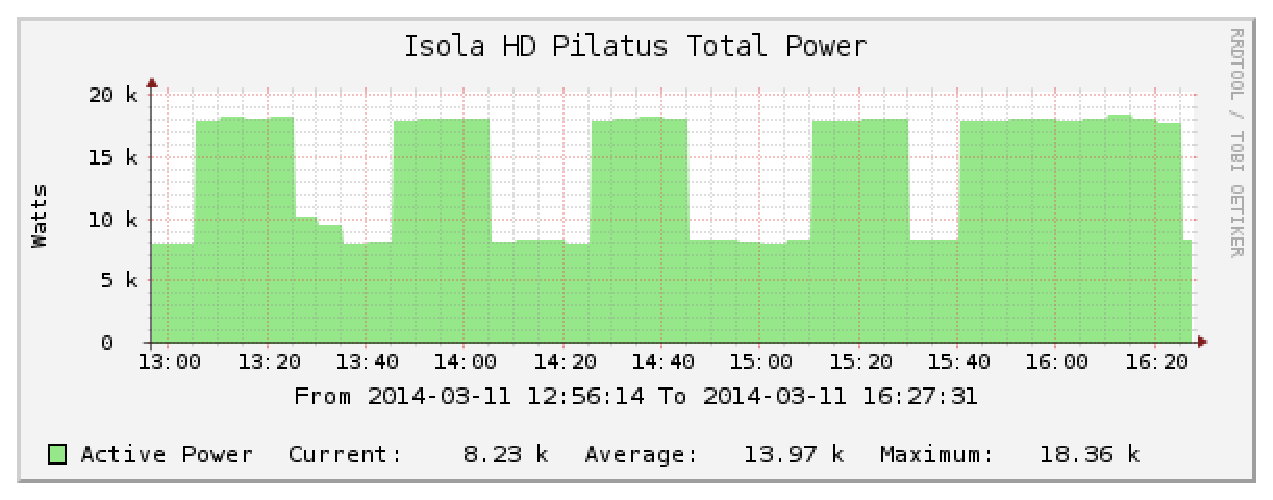
\includegraphics[width=0.48\textwidth]{Figs/NRJ_benchmark_Pilatus.eps}
    \caption{Pilatus: Isola HD Total Power}
    \label{fig:2}
  \end{center}
\end{figure}

Figures~\ref{fig:1} and  \ref{fig:2} account respectively  for Monch's
Isola E1  Rack 2  and Pilatus' Isola  HD total power  measurements for
1-day or 2-days simulations. On  the Intel Ivy Bridge EP based cluster
(i.e. Monch), the 1-day simulation  was issued only twice due to usage
restrictions. As time resolution was set to one update every 5 minutes
for  power sampling,  the average  power consumption  was  computed by
considering 6 values for each single  run.  On the Intel Xeon E5 based
cluster (i.e.   Pilatus), the 1-day  simulation was issued  four times
and a 2-days  run only once. Similarly, the  average power consumption
was computed by  considering 4 values for each single  1-day run and 9
values  for the  2-days  run. Corresponding  results  are gathered  in
Table~\ref{tab:3}.

\begin{table}[htbf]
  \begin{center}
    \caption{Average power consumption (W) of the platforms}
    \label{tab:3}
    \begin{tabular}{ccc}
      \hline\noalign{\smallskip}
      \textbf{Simulation time} & \textbf{Xeon E5} & \textbf{Ivy Bridge EP} \\
      \noalign{\smallskip}\hline\noalign{\smallskip}
      \textbf{1 day} & 18122.01417 & 12658.52278 \\ 
      & 17979.61083 & 12586.40833 \\
      & 18065.45167 & - \\
      & 17973.02833 & - \\
      \noalign{\smallskip}\hline\noalign{\smallskip}
      \textbf{2 days} & 17997.57815 & - \\
      \noalign{\smallskip}\hline
    \end{tabular}
  \end{center}
\end{table}

In Figure~\ref{fig:3}, we compare both time-to-solution (right y-axis)
and  energy-to-solution (left  y-axis) metrics  on both  platforms. As
expected,  Xeon  E5 outperforms  Ivy  Bridge  EP,  being roughly  1.3x
faster.   The reason for  that is  two-fold: (1)  it has  higher clock
frequency than Ivy  Bridge (2.6 GHz against 2.2 GHz),  and (2) it aims
at  computing   speed  regardless   to  energy  consumption.   In  our
experiments,  Ivy  Bridge   EP  showed  the  best  energy-to-solution,
reducing the energy consumption of Xeon E5 by approximately $7\%$.

\begin{figure}[htbf]
  \includegraphics[width=0.5\textwidth]{Figs/Time_E2S_COSMO-ART-0.eps}
  \caption{Time-to-solution and energy-to-solution comparison between
    Xeon E5 and Ivy Bridge-EP architectures}
  \label{fig:3}
\end{figure}

\begin{figure}[htbf]
  \includegraphics[width=0.5\textwidth]{Figs/Time_E2S_COSMO-ART-1.eps}
  \caption{Time-to-solution and energy-to-solution on Tintorrum -
    Polling mode}
  \label{fig:3}
\end{figure}

\begin{figure}[htbf]
  \includegraphics[width=0.5\textwidth]{Figs/Time_E2S_COSMO-ART-2.eps}
  \caption{Time-to-solution and energy-to-solution on Tintorrum -
    Blocking mode}
  \label{fig:3}
\end{figure}


\section{Conclusion \emph{(to be completed)}}
\label{concl}
We  have   presented  a  methodology  for   comparing  performance  of
COSMO-ART,  a  regional  weather  forecast  model  augmented  for  the
interactions of  reactive gases and aerosol  particles.  The resulting
benchmarks illustrate  that the  best time-to-solution does  not imply
the best energy-to-solution: an Intel Sandybridge (2.6 GHz) system has
lower  time-to-solution but  higher energy-to-solution  than  an Intel
Ivybridge  (2.2  GHz) system,  although  the  two  metrics are  indeed
strongly  correlated. On the other hand, the usage of energy-friendly MPI waiting techniques analzyed with our power-performance framework over a series of runs of \cosmoart on \tinto and
power traces demonstrate that it is possible to reduce both
power dissipation and energy-to-solution while maintaining (or even decreasing) the time-to-solution. The  resulting profiles indicate that simple
changes, such as making use of the blocking MPI policy rather
than the polling is possible to slightly reduce both power dissipation and energy consumption (by 2\,\%).

This  reproducible  benchmark provides  a  baseline  for ongoing  work
package within  the EU-funded Exa2Green to  minimise power consumption
of COSMO-ART. Profiling  has given us insight into  the most expensive
code  components,  which are  now  being  altered  to utilise  revised
algorithms.  The  results of these  optimisations will be  reported in
future publications.


%\paragraph{Paragraph headings} Use paragraph headings as needed.

\begin{acknowledgements}
The research  leading to these  results is supported by  the Exa2Green
project  co-financed by  the European  Commission under  7th Framework
Programme Future and Emerging Technologies (FET) Proactive Initiative:
Minimising Energy  Consumption of Computing to the  Limit (MINECC). We
also gratefully acknowledge the High Performance and High Productivity
Computing  Initiative  (\url{www.hp2c.ch}) for  results  that will  be
leveraged in subsequent code refactoring.
\end{acknowledgements}

\DeclareRobustCommand\IPCClongname{ - Intergovernmental Panel on Climate Change}

\bibliographystyle{plainnat}
\bibliography{\jobname}

\end{document}

